\documentclass[a5paper]{article}

\usepackage{amsmath, amssymb}
\usepackage{multicol}
\setlength{\columnsep}{1cm}
\usepackage[margin=0.75in]{geometry}
\usepackage{graphicx}
\graphicspath{ {../../../Images/ENEE12014/} }
\usepackage[breaklinks, hidelinks]{hyperref}
\usepackage{siunitx}
\usepackage{tikz}
\usetikzlibrary{positioning, arrows.meta}
\usepackage[american]{circuitikz}
\usepackage{pgfplots}
\pgfplotsset{compat=newest}
\usepgfplotslibrary{external}
\usepackage{stix}
\usepackage{ragged2e}
\usepackage{enumitem}
\usepackage{polynom}

\newcommand{\sech}{\mathrm{sech}}
\newcommand{\csch}{\mathrm{csch}}
\setcounter{secnumdepth}{4}
\renewcommand\paragraph{\@startsection{paragraph}{4}{\z@}%
% display heading, like subsubsection
                                     {-3.25ex\@plus -1ex \@minus -.2ex}%
                                     {1.5ex \@plus .2ex}%
                                     {\normalfont\normalsize\bfseries}}
\sisetup{
	round-mode = places,
	round-precision = 2,
}

\date{19\textsuperscript{th} of June 2026}

\begin{document}
	\begin{titlepage}
		\centering
		{\Huge \textsc{COIT12209}\par}
		\vspace{1cm}
		{\Large \textsc{Lecture Notes}\par}
		\vspace{2.5cm}
		\vfill
		Authored by\par
		Lachlan J. W. Wyer
		\vfill
		\makeatletter
		{\large Document Start Date: \@date \par}
		\makeatother
		{\large Latest Update: \today\par}
	\end{titlepage}
	\tableofcontents
	\pagebreak

	\section{Introduction}
	\subsection{Electricity:}
	Through this is a steady of moving charges and their interaction until magnetic and electric fields change this. Charges move because a net force have been applied. The force comes from a difference in charge between two points on a circuit.
	\subsection{SI Units:}
	$$1\;Coulomb=6.25\times10^{18}e^{-}$$
	$$1A=\frac{1Q(Coulomb)}{1t(Seconds)}$$
	\subsection{Electrical Potential Energy:}
	The potential energy is closely associated with an object's position. $E_{PE}$ is what all electrical circuits have. To move charges within an electric field it requires an amount of work.
	\subsection{Voltage:}
	$$1V=\frac{1J}{C}$$
	Defines the potential difference between two points in a conductor.
	\subsection{Elctro Motive Force:}
	emf is the energy provided by an eneyr source to enable the flow of charges.
	\subsection{Grounding:}
	When grounding a circuit we are basically joining it a giant resvior of both positive and negative charge. This is large enough that it can both recieve and donate charge. As such when an object comes into contact with group all net charge is removed becoming something with OV.
	\begin{center}
	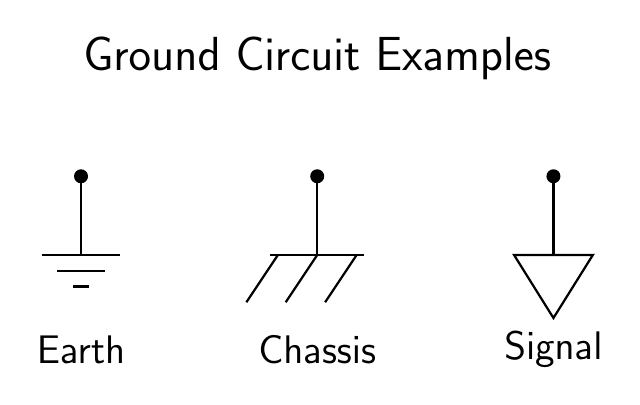
\begin{tikzpicture}[
	    thick,
	    % Style for the connection dots
	    terminal/.style={circle, fill=black, inner sep=1.5pt, draw}
	]

	% Title
	\node[font=\LARGE\sffamily] at (3, 1.5) {Ground Circuit Examples};

	% -----------------
	% Earth Ground
	% -----------------
	\begin{scope}[xshift=0cm]
	    \node[terminal] at (0,0) {};
	    % Vertical line
	    \draw (0,0) -- (0,-1);
	    % Horizontal lines
	    \draw (-0.5,-1) -- (0.5,-1);
	    \draw (-0.3,-1.2) -- (0.3,-1.2);
	    \draw (-0.1,-1.4) -- (0.1,-1.4);
	    % Label
	    \node[font=\Large\sffamily] at (0, -2.2) {Earth};
	\end{scope}

	% -----------------
	% Chassis Ground
	% -----------------
	\begin{scope}[xshift=3cm]
	    \node[terminal] at (0,0) {};
	    % Vertical line
	    \draw (0,0) -- (0,-1);
	    % Horizontal line
	    \draw (-0.6,-1) -- (0.6,-1);
	    % Diagonal hash lines
	    \draw (-0.5,-1) -- (-0.9,-1.6);
	    \draw (0,-1) -- (-0.4,-1.6);
	    \draw (0.5,-1) -- (0.1,-1.6);
	    % Label
	    \node[font=\Large\sffamily] at (0, -2.2) {Chassis};
	\end{scope}

	% -----------------
	% Signal Ground
	% -----------------
	\begin{scope}[xshift=6cm]
	    \node[terminal] at (0,0) {};
	    % Vertical line
	    \draw (0,0) -- (0,-1);
	    % Triangle
	    \draw (-0.5,-1) -- (0.5,-1) -- (0,-1.8) -- cycle;
	    % Label
	    \node[font=\Large\sffamily] at (0, -2.2) {Signal};
	\end{scope}
	\end{tikzpicture}
	\end{center}
	\subsection{Passive Circuit Element:}
	Conductors are circuit elements that allow the free movement of charge. Super conductors do this with no resistance. Insulators are the opposite of conductors. They prevent the free movement of charge. A semi-conductor has properties of conductors and insulators.
	\subsection{Resistance:}
	Resistivity ($\rho$) is how strongly it resists electrical current.
	$$R=\frac{\rho L}{A}$$
	Where:
	\begin{itemize}
		\item R: Resistance ($\Omega$)
		\item $\rho$: Resistivity ($(\Omega\cdot m)^{-1}$)
		\item L: Lenght of wire ($m$)
		\item A: CSA ($m^{2}$)
	\end{itemize}
	\subsection{Circuit Symbols:}
	\begin{center}
	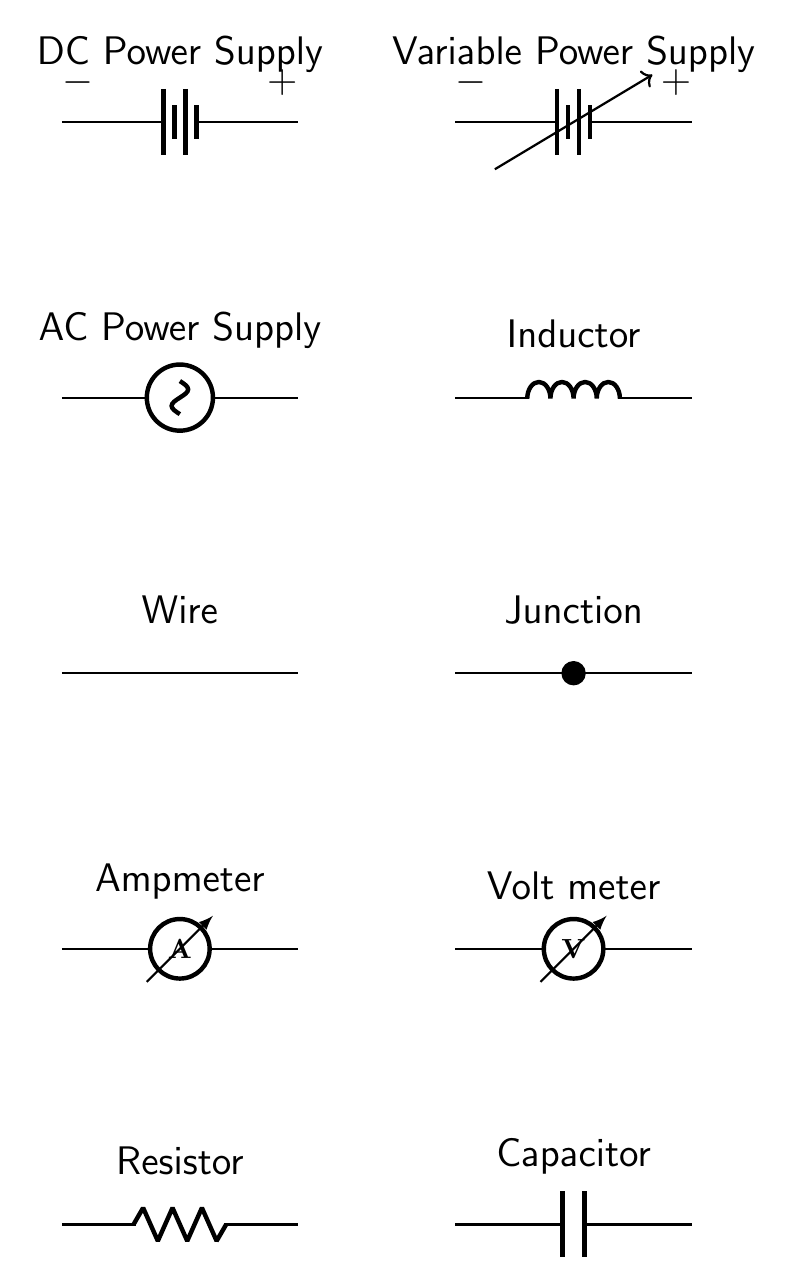
\begin{tikzpicture}[
	    label/.style={font=\Large\sffamily, align=center},
	    thick
	]

	% DC Power Supply
	\begin{scope}[shift={(0, 0)}]
	    \node[label, anchor=south] at (0, 0.5) {DC Power Supply};
	    \draw (-1.5, 0) to[battery] (1.5, 0);
	    \node[font=\Large] at (-1.3, 0.5) {$-$};
	    \node[font=\Large] at (1.3, 0.5) {$+$};
	\end{scope}

	% Variable Power Supply
	\begin{scope}[shift={(5, 0)}]
	    \node[label, anchor=south] at (0, 0.5) {Variable Power Supply};
	    \draw (-1.5, 0) to[battery] (1.5, 0);
	    % Arrow indicating variable tuning
	    \draw[->] (-1, -0.6) -- (1, 0.6);
	    \node[font=\Large] at (-1.3, 0.5) {$-$};
	    \node[font=\Large] at (1.3, 0.5) {$+$};
	\end{scope}

	% AC Power Supply
	\begin{scope}[shift={(0, -3.5)}]
	    \node[label, anchor=south] at (0, 0.5) {AC Power Supply};
	    \draw (-1.5, 0) to[sV] (1.5, 0);
	\end{scope}

	% Inductor
	\begin{scope}[shift={(5, -3.5)}]
	    \node[label, anchor=south] at (0, 0.5) {Inductor};
	    \draw (-1.5, 0) to[L] (1.5, 0);
	\end{scope}

	% Wire
	\begin{scope}[shift={(0, -7)}]
	    \node[label, anchor=south] at (0, 0.5) {Wire};
	    \draw (-1.5, 0) -- (1.5, 0);
	\end{scope}

	% Junction
	\begin{scope}[shift={(5, -7)}]
	    \node[label, anchor=south] at (0, 0.5) {Junction};
	    \draw (-1.5, 0) -- (1.5, 0);
	    \filldraw (0, 0) circle (4pt);
	\end{scope}

	% Ampmeter
	\begin{scope}[shift={(0, -10.5)}]
	    \node[label, anchor=south] at (0, 0.5) {Ampmeter};
	    \draw (-1.5, 0) to[ammeter] (1.5, 0);
	\end{scope}

	% Volt meter
	\begin{scope}[shift={(5, -10.5)}]
	    \node[label, anchor=south] at (0, 0.5) {Volt meter};
	    \draw (-1.5, 0) to[voltmeter] (1.5, 0);
	\end{scope}

	% Resistor
	\begin{scope}[shift={(0, -14)}]
	    \node[label, anchor=south] at (0, 0.5) {Resistor};
	    \draw (-1.5, 0) to[R] (1.5, 0);
	\end{scope}

	% Capacitor
	\begin{scope}[shift={(5, -14)}]
	    \node[label, anchor=south] at (0, 0.5) {Capacitor};
	    \draw (-1.5, 0) to[C] (1.5, 0);
	\end{scope}

	\end{tikzpicture}
	\end{center}
	\pagebreak
	Voltage rises across from the negative to positive terminals of the components. In addition to the opposite flow to the amps. Current divider rule:
	$$I_{1}=I_{S}\cdot\frac{R_{2}}{R_{1}+R_{2}}$$
	$$I_{2}=I_{S}\cdot\frac{R_{1}}{R_{1}+R_{2}}$$
	
	\section{Circuit Simplification}
	\subsection{Ideal Power Sources:}
	For ideal voltage and current sources, there are independent and dependent sources. The independent source are illustrated by a circle around the indicator and its numerical value is just defined. The dependent source usually rely on a contast multiplied by a either a current or voltage value within the circuit. They are also illustrated through a diamond shape.
	\subsection{Polarity and Power:}
	\begin{center}
	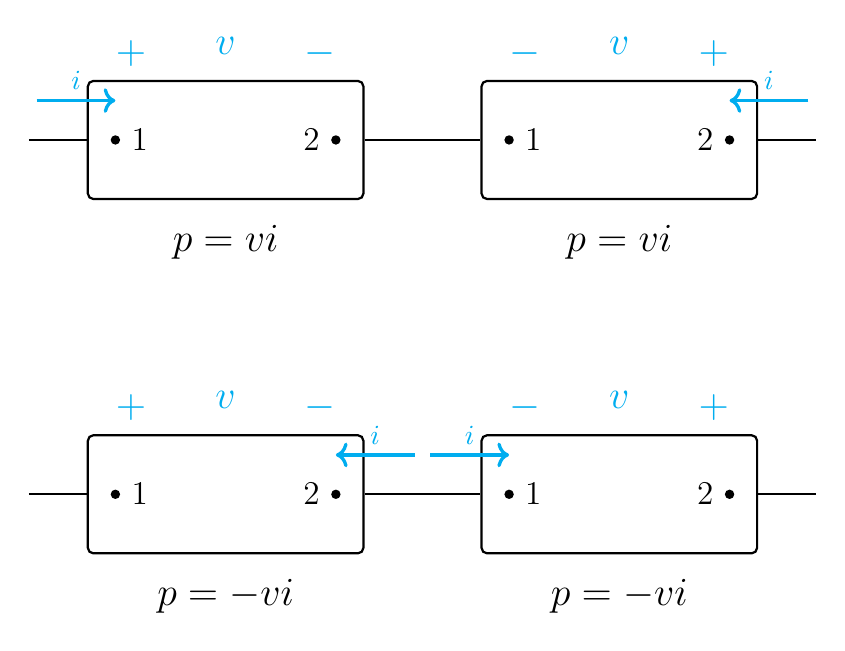
\begin{tikzpicture}[
	    thick,
	    % Styles for the components
	    box/.style={draw, thick, minimum width=3.5cm, minimum height=1.5cm, rounded corners=2pt},
	    terminal/.style={circle, fill=black, inner sep=1.2pt},
	    annotation/.style={text=cyan, font=\Large},
	    arrow/.style={->, cyan, very thick}
	]

	% =========================
	% Top Left Diagram
	% =========================
	\begin{scope}[shift={(0,0)}]
	    % Box and wires
	    \node[box] (b1) at (0,0) {};
	    \draw (-2.5, 0) -- (b1.west);
	    \draw (b1.east) -- (2.5, 0);

	    % Terminals
	    \node[terminal, label=right:{\large 1}] at (-1.4, 0) {};
	    \node[terminal, label=left:{\large 2}] at (1.4, 0) {};

	    % Annotations (Voltage & Current)
	    \node[annotation] at (-1.2, 1.1) {$+$};
	    \node[annotation] at (1.2, 1.1) {$-$};
	    \node[annotation] at (0, 1.2) {$v$};

	    \draw[arrow] (-2.4, 0.5) -- (-1.4, 0.5) node[midway, above, text=cyan] {$i$};

	    % Equation
	    \node[font=\Large] at (0, -1.3) {$p = vi$};
	\end{scope}

	% =========================
	% Top Right Diagram
	% =========================
	\begin{scope}[shift={(5,0)}]
	    % Box and wires
	    \node[box] (b2) at (0,0) {};
	    \draw (-2.5, 0) -- (b2.west);
	    \draw (b2.east) -- (2.5, 0);

	    % Terminals
	    \node[terminal, label=right:{\large 1}] at (-1.4, 0) {};
	    \node[terminal, label=left:{\large 2}] at (1.4, 0) {};

	    % Annotations (Voltage & Current)
	    \node[annotation] at (-1.2, 1.1) {$-$};
	    \node[annotation] at (1.2, 1.1) {$+$};
	    \node[annotation] at (0, 1.2) {$v$};

	    \draw[arrow] (2.4, 0.5) -- (1.4, 0.5) node[midway, above, text=cyan] {$i$};

	    % Equation
	    \node[font=\Large] at (0, -1.3) {$p = vi$};
	\end{scope}

	% =========================
	% Bottom Left Diagram
	% =========================
	\begin{scope}[shift={(0,-4.5)}]
	    % Box and wires
	    \node[box] (b3) at (0,0) {};
	    \draw (-2.5, 0) -- (b3.west);
	    \draw (b3.east) -- (2.5, 0);

	    % Terminals
	    \node[terminal, label=right:{\large 1}] at (-1.4, 0) {};
	    \node[terminal, label=left:{\large 2}] at (1.4, 0) {};

	    % Annotations (Voltage & Current)
	    \node[annotation] at (-1.2, 1.1) {$+$};
	    \node[annotation] at (1.2, 1.1) {$-$};
	    \node[annotation] at (0, 1.2) {$v$};

	    \draw[arrow] (2.4, 0.5) -- (1.4, 0.5) node[midway, above, text=cyan] {$i$};

	    % Equation
	    \node[font=\Large] at (0, -1.3) {$p = -vi$};
	\end{scope}

	% =========================
	% Bottom Right Diagram
	% =========================
	\begin{scope}[shift={(5,-4.5)}]
	    % Box and wires
	    \node[box] (b4) at (0,0) {};
	    \draw (-2.5, 0) -- (b4.west);
	    \draw (b4.east) -- (2.5, 0);

	    % Terminals
	    \node[terminal, label=right:{\large 1}] at (-1.4, 0) {};
	    \node[terminal, label=left:{\large 2}] at (1.4, 0) {};

	    % Annotations (Voltage & Current)
	    \node[annotation] at (-1.2, 1.1) {$-$};
	    \node[annotation] at (1.2, 1.1) {$+$};
	    \node[annotation] at (0, 1.2) {$v$};

	    \draw[arrow] (-2.4, 0.5) -- (-1.4, 0.5) node[midway, above, text=cyan] {$i$};

	    % Equation
	    \node[font=\Large] at (0, -1.3) {$p = -vi$};
	\end{scope}
	\end{tikzpicture}
	\end{center}
	\subsection{Voltage Divider Rule:}
	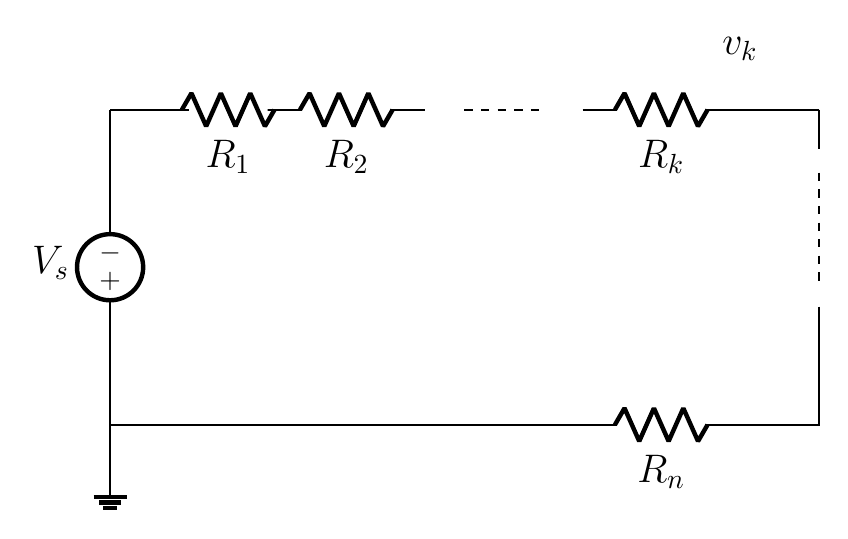
\begin{tikzpicture}[thick, font=\Large]
	    % Voltage Source and Ground
	    \draw (0,0) to[V, l=$V_s$] (0,4);
	    \draw (0,0) -- (0,-0.5) node[ground]{};

	    % Top branch (R1 and R2)
	    \draw (0,4) -- (1,4)
		to[R, l_=$R_1$] (2,4)
		to[R, l_=$R_2$] (4,4);

	    % Dashed continuation (horizontal)
	    \draw[dashed] (4.5, 4) -- (5.5, 4);

	    % R_k with v_k label above
	    \draw (6,4) to[R, l_=$R_k$] (8,4) -- (9,4);
	    \node[above] at (8, 4.5) {$v_k$};

	    % Right side dashed gap (vertical)
	    \draw (9,4) -- (9, 3.5);
	    \draw[dashed] (9, 3.2) -- (9, 1.8);
	    \draw (9, 1.5) -- (9, 1);

	    % Bottom branch returning to source (R_n)
	    \draw (0,0) -- (6,0) 
		to[R, l_=$R_n$] (8,0) -- (9,0) -- (9,1);
	\end{tikzpicture}\\
	For this to work the current through all resistors must be equal. The highest voltage drop occurs over the largest resistor. 
	$$V_{k}=\frac{R_{k}}{R_{eq}}\cdot V_{S}$$
	\subsection{Current Divider Rule:}
	\begin{center}
	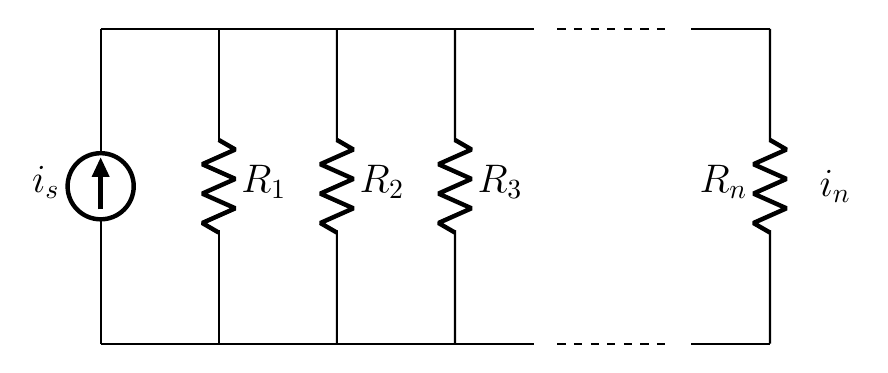
\begin{tikzpicture}[thick, font=\Large]
	    % Current Source (i_s)
	    \draw (0,0) to[I, l=$i_s$] (0,4);

	    % Top and Bottom continuous wires
	    \draw (0,4) -- (5.5,4);
	    \draw (0,0) -- (5.5,0);

	    % Parallel Resistors R1, R2, R3
	    \draw (1.5,4) to[R, l=$R_1$] (1.5,0);
	    \draw (3,4) to[R, l=$R_2$] (3,0);
	    \draw (4.5,4) to[R, l=$R_3$] (4.5,0);

	    % Dashed lines for continuation gap
	    \draw[dashed] (5.8, 4) -- (7.2, 4);
	    \draw[dashed] (5.8, 0) -- (7.2, 0);

	    % Final segment and Rn
	    \draw (7.5,4) -- (8.5,4);
	    \draw (7.5,0) -- (8.5,0);
	    \draw (8.5,4) to[R, l_=$R_n$] (8.5,0);

	    % i_n label next to the last branch
	    \node[right] at (9, 2) {$i_n$};
	\end{tikzpicture}
	\end{center}
	The highest current goes through the smallest resistor.
	$$I_{k}=\frac{I_{S}}{R_{k}R_{eq}}$$
	\subsection{Delta-Wye Resistor Configurations:}
	\begin{center}
		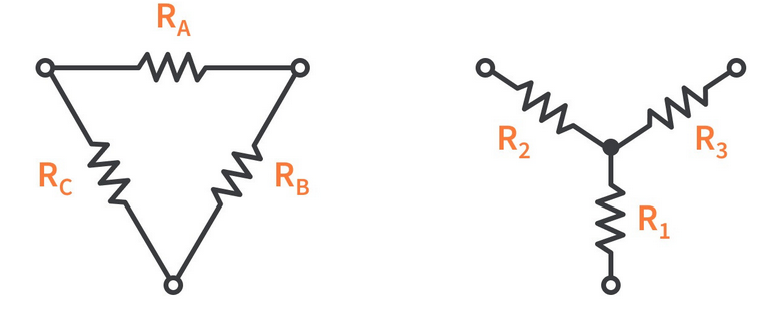
\includegraphics[scale=0.75]{delta-wye.png}
	\end{center}
	\begin{align*}
		R_{a}=&\frac{R_{1}R_{2}+R_{2}R_{3}+R_{3}R_{1}}{R_{1}} & R_{1}=&\frac{R_{b}R_{c}}{R_{a}+R_{b}+R_{c}}\\
		R_{b}=&\frac{R_{1}R_{2}+R_{2}R_{3}+R_{3}R_{1}}{R_{2}} & R_{2}=&\frac{R_{c}R_{a}}{R_{a}+R_{b}+R_{c}}\\
		R_{c}=&\frac{R_{1}R_{2}+R_{2}R_{3}+R_{3}R_{1}}{R_{3}} & R_{3}=&\frac{R_{a}R_{b}}{R_{a}+R_{b}+R_{c}}
	\end{align*}

	\section{Nodal Analysis}
	\subsection{Planar Circuit:}
\end{document}
